
\newpage

\section*{Soluzione}

\subsection*{Es. 1}

La cooperazione tra frammenti di programmi scritti in linguaggi
diversi pu\`o essere difficoltosa a causa delle diverse convenzioni
nell'utilizzo dei registri macchina, dello \emph{stack}, nella
rappresentazione dei tipi numerici ecc. Per limitare questo tipo di
problemi \`e possibile specificare le convenzioni di collegamento da
utilizzare in una chiamata \cpp{extern}. In particolare, la direttiva
\cpp{extern ``C''} \`e quella utilizzata per collegare frammenti di
codice C, assembler e Fortran, tutti conformi alle medesime
convenzioni. La direttiva \cpp{extern ``C''} pu\`o essere specificata
per un insieme di dichiarazioni raggruppate in uno \emph{blocco di
  collegamento}:
\begin{lstlisting}
extern "C" {
    char* strcpy(char*, const char*);
    int strlen(const char*);
}
\end{lstlisting}
Di seguito si riporta il listato della classe \emph{wrapper}
\cpp{lapack::TriDiag}, che fattorizza e risolve un sistema lineare
tridiagonale utilizzando le \emph{routine} Lapack \cpp{dgttrf} e
\cpp{dgttrs}\footnote{Le \emph{routine} Lapack sono documentate anche
  da \emph{man page} cui si accede, da linea di comando, digitando
  \texttt{man} seguito dal nome della \emph{routine}.}. 
\lstset{basicstyle=\scriptsize\sf}
\lstinputlisting{./es/1/tridiag.hpp}
\lstset{basicstyle=\sf}

Secondo la convenzione, i nomi Fortran vengono modificati nel file
oggetto aggiungendo il carattere di sottolineatura alla fine. Nel
codice proposto tale traslitterazione \`e operata automaticamente
dalla macro \cpp{F77NAME} che, applicata all'argomento \cpp{X},
restituisce \cpp{X_}. Si noti, poi, che gli argomenti di tipo intero
delle \emph{routine} Fortran sono, in effetti, delle referenze a
\cpp{int}. La ragione \`e che, in Fortran, tutti gli argomenti vengono
passati per indirizzo: se avessimo, quindi, dichiarato tali argomenti
come \cpp{int} anzich\'e come \cpp{int&}, il valore passato sarebbe
stato erroneamente interpretato come un indirizzo. 

L'implementazione della classe \emph{wrapper} \`e collocata
all'interno del \emph{namespace} \cpp{lapack}. L'uso di un
\emph{namespace} contribuisce a migliorare l'organizzazione di un
codice. Si supponga, inoltre, di disporre di un'altra implementazione
di un solutore di Thomas: quest'ultima potrebbe essere accessibile
mediante un'altra classe \cpp{TriDiag} contenuta in un diverso
\emph{namespace}. In tal caso, se le interfacce fossero compatibili,
si potrebbe passare da un'implementazione all'altra semplicemente
specificando il \emph{namespace} desiderato. 

Gli argomenti da passare alle \emph{routine} Fortran sono memorizzati
in membri \cpp{private} della classe, in modo da nascondere i dettagli
implementativi all'utente. La classe accede ai vettori contenenti gli
elementi delle tre diagonali della matrice mediante i tre iteratori
passati al costruttore. Il tipo dell'iteratore \`e parametro
\cpp{template} per la classe. Qualora si utilizzino dei
vettori in stile C, il tipo dell'iteratore 
sar\`a \cpp{double*}, ovvero puntatore a \cpp{double}: baster\`a,
quindi, passare il nome dell'\emph{array}. Qualora si vogliano usare
degli \cpp{std::vector<double>}, il tipo corretto per \cpp{Iterator}
sarebbe \cpp{std::vector<double>::iterator}. In ogni caso, il tipo
fornito come parametro \cpp{template} deve obbedire ad una
\emph{policy}: deve soddisfare le specifiche dell'algebra dei
puntatori. Al compilatore \`e richiesto di risolvere il tipo
dell'iteratore, controllando che soddisfi i requisiti sintattici.

Nel costruttore della classe \cpp{TriDiag} i vettori \cpp{a}, \cpp{b}
e \cpp{c} passati come argomenti vengono copiati nei membri
\cpp{M_dl}, \cpp{M_d__} e \cpp{M_du} della classe. Per la copia si
sfruttano l'algebra dei puntatori e l'operatore di
dereferenziazione. Si noti che l'assegnazione \cpp{p = M_dl} \`e
lecita in quanto il nome di un vettore \`e, in effetti, un puntatore
al primo elemento. Incrementando \cpp{p} mediante l'istruzione
\cpp{++p} si ottiene un puntatore all'elemento successivo del
vettore. Il punto critico in questo meccanismo di copia risiede nel
fatto che l'accesso al vettore avviene senza \emph{boundary check}, e
si potrebbero verificare accessi \emph{out of bounds} qualora si
sbagli a specificare la condizione di uscita dal ciclo. Nella
documentazione della classe viene indicata esplicitamente una
\emph{precondizione} per le variabili di tipo \cpp{Iterator}: \`e compito
dell'utilizzatore di \cpp{TriDiag} garantire che l'iteratore punti ad
un'area di memoria della giusta dimensione. Sempre nel
costruttore viene richiamata la \emph{routine} Lapack \cpp{dgttrf} che
effettua la fattorizzazione della matrice. 

Da notare \`e anche l'uso delle asserzioni, che verificano se si sono
avuti dei problemi nell'allocazione della memoria. La funzione
\cpp{assert} costituisce il pi\`u semplice strumento di
\emph{controllo dell'eccezioni}.

Nel membro \cpp{TriDiag::solve} c'\`e da notare che il valore
dell'iteratore \cpp{rhs} viene memorizzato all'inizio della
procedura. In questo modo la variabile \cpp{rhs} pu\`o essere
aggiornata con la soluzione del sistema lineare. Il puntatore a
\cpp{double} \cpp{b} \`e una variabile di supporto da fornire alla
routine Fortran. 

Il distruttore ed il membro \cpp{TriDiag::status} sono implementati
separatamente nel file \cpp{tridiag.cpp}. Tale file pu\`o essere
compilato una sola volta mediante l'istruzione seguente: 
\begin{verbatim}
g++ -c tridiag.cpp
\end{verbatim}
Il file oggetto \texttt{tridiag.o} cos\`i ottenuto pu\`o essere
successivamente collegato come segue: 
\begin{verbatim}
g++ fin.cpp tridiag.o -llapack -o fin.exe
\end{verbatim}

Si riporta di seguito il codice per il problema dell'aletta modificato
secondo le indicazioni del testo. 
\lstset{basicstyle=\scriptsize\sf}
\lstinputlisting{./es/1/fin.cpp}
\lstset{basicstyle=\sf}
I dati del problema vengono letti da file utilizzando la libreria
GetPot, che offre anche strumenti per l'analisi logica
dell'\emph{input} da linea di comando. GetPot supporta
l'organizzazione per sezioni del file di dati, secondo il modello
seguente: 
\lstset{basicstyle=\scriptsize\sf}
\lstinputlisting{./es/1/data.pot}
\lstset{basicstyle=\sf}
La sintassi \`e molto semplice: il nome della sezione \`e racchiuso
tra parentesi quadre ed \`e relativo alla posizione precedente. Nel
caso d'esempio si hanno tre sezioni (\cpp{mesh}, \cpp{geometry} e
\cpp{physics}) sullo stesso livello. Se in luogo di
\cpp{[../geometry]} avessimo cominciato la sezione con l'\emph{header}
\cpp{[./geometry]}, questa sarebbe divenuta una sottosezione di
\cpp{mesh}, accessibile mediante il prefisso
\cpp{mesh/geometry}. L'utilizzo di GetPot in un codice C++ richiede la
definizione di un'istanza dell'oggetto \cpp{GetPot} inizializzata con
il nome del file di dati. Nel nostro caso: 
\begin{lstlisting}
GetPot ifile(``data.pot'');
\end{lstlisting}
% \begin{figure}
% \begin{minipage}{0.5\textwidth}
% \centering
% \subfigure[File di dati]{\lstinputlisting{getpot_sample.pot}}
% \end{minipage}
% \begin{minipage}{0.5\textwidth}
% \centering
% \subfigure[Struttura logica (nomi di sezione in grassetto).]{
% \psfrag{vehicle}{{\bf vehicle}}
% \psfrag{length}{length}
% \psfrag{initial-xyz}{initial-xyz}
% \psfrag{tires}{{\bf tires}}
% \psfrag{front}{{\bf front}}
% \psfrag{back}{{\bf back}}
% \psfrag{right}{{\bf right}}
% \psfrag{left}{{\bf left}}
% \psfrag{chassis}{{\bf chassis}}
% \psfrag{Rho}{rho}
% \psfrag{S}{S}
% \psfrag{Cd}{Cd}
% \psfrag{B}{B}
% \psfrag{C}{C}
% \psfrag{D}{D}
% \psfrag{E}{E}
% 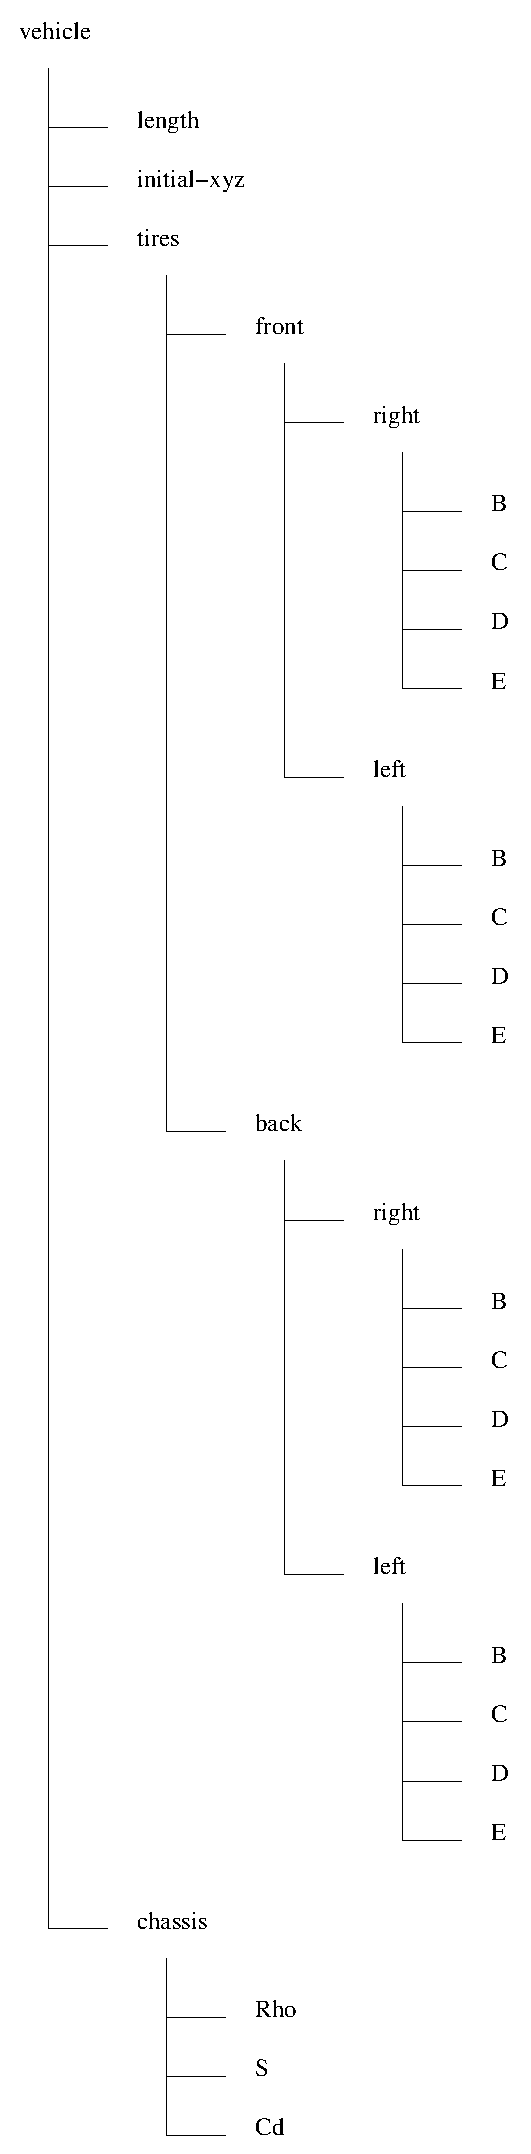
\includegraphics[height=120mm]{./figures/eps/getpot_sample.eps}
% }
% \end{minipage}
% \caption{Esempio di file dati per GetPot.}
% \label{fig:getpot_sample}
% \end{figure}
% Un esempio pi\`u elaborato \`e riportato in %\figref{fig:getpot_sample}.
Le variabili vengono lette mediante l'\cpp{operator()} della classe \cpp{GetPot} passando due argomenti:
\begin{itemize}
\item una stringa di caratteri contenente il nome completo della variabile (percorso incluso);
\item un valore di default che viene utilizzato qualora la variabile non sia stata rintracciata nel file dati.
\end{itemize}
Dovendo leggere pi\`u variabili da una medesima sezione \`e possibile specificare il prefisso mediante il membro \cpp{set_prefix}.

\subsection*{Es. 2}

Il contenitore associativo \cpp{std::map} consente di descrivere un
insieme in cui ad ogni occorrenza di una certa \emph{chiave}
corrisponde in modo univoco un \emph{valore}. Per soddisfare la prima
richiesta dell'esercizio si pu� utilizzare un contenitore di questo tipo, nel quale la
chiave sia l'identificatore del nodo della mesh mentre il valore sia la
stringa che definisce la condizione al bordo associata.

Un contenitore \cpp{std::multimap} pu� essere utile invece qualora si
voglia gestire l'insieme di nodi associati a ciascuna condizione al
contorno: in questo caso la chiave della multimappa � la stringa (nome
della condizione al bordo) mentre i valori associati (possono essere
pi� di uno) sono gli identificativi dei nodi.

\lstset{basicstyle=\scriptsize\sf}
\lstinputlisting[caption=Classe \cpp{Mesh}: definizione di una mappa e
di una multimappa STL.,
linerange={31-37,40-42,70-70,75-80}]{./es/2/src/mesh.hpp}
\lstset{basicstyle=\sf}

L'operazione di inserimento efficiente di elementi in \cpp{std::map} e
\cpp{std::multimap} richiede il ricorso alla funzione
\cpp{make\_pair}, che crea un oggetto \cpp{pair} di tipo compatibile
con il generico elemento della mappa:

\lstset{basicstyle=\scriptsize\sf}
\lstinputlisting[caption=Costruttore di \cpp{Mesh}: inserimento di
elementi nelle mappe., linerange={3-7,17-32,61-61}]{./es/2/src/mesh.cpp}
\lstset{basicstyle=\sf}

\`E possibile sfruttare la sintassi dell'operatore di \emph{subscript}
(\cpp{operator[]}) per popolare la mappa:
\begin{lstlisting}
  M_boundary_points[ i ]= bc;
\end{lstlisting}
tuttavia questa istruzione fa s\`i che, quando la mappa \`e vuota,
ciascun valore sia inizializzato ad un valore di default e poi gli sia
assegnato il valore esplicito. Se i valori sono istanze di una classe per la
quale inizializzazione di default e assegnamento siano operazioni
onerose, le prestazioni del programma possono essere ridotte.

L'operatore di \emph{subscript} viene utilizzato per l'accesso agli elementi memorizzati:
\lstset{basicstyle=\scriptsize\sf}
\lstinputlisting[caption=Operatore di scorrimento per \cpp{Mesh}:
accesso ai valori in mappe
STL., linerange={63-64,66-74,81-84}]{./es/2/src/mesh.cpp}
\lstset{basicstyle=\sf}

La ricerca degli identificatori dei nodi associati ad una certa
condizione al bordo si realizza applicando opportuni \cpp{algoritmi}
(forniti dall'\emph{header file} \cpp{algorithm})
ai contenitori STL.

Se si lavora con la mappa \cpp{M_boundary_points}, si pu� utilizzare
l'algoritmo STL \cpp{find_if}: scandisce gli elementi della mappa
compresi tra gli iteratori forniti come primo e secondo parametro, ed
applica a ciascun elemento il \emph{predicato} (cio\`e una funzione il
cui risultato rappresenta il valore di verit\`a di una certa
condizione) passato come terzo argomento. Nel caso considerato, il
\emph{predicato} \`e rappresentato dal \emph{funtore} \cpp{value_equals}:
una classe con \cpp{operator()} sovraccaricato e definito in modo da
confrontare il valore di ciascun elemento della mappa con il valore
desiderato.

\lstset{basicstyle=\scriptsize\sf}
\lstinputlisting[caption=Funtore
\cpp{value_equals}., linerange={16-31}]{./es/2/src/mesh.hpp}
\lstset{basicstyle=\sf}

L'algoritmo di stampa a schermo degli identificativi dei nodi
associati ad una certa condizione al bordo � quello riportato di seguito:

\begin{lstlisting}
  // Print out points having a given boundary condition
  void Mesh::bc( std::string const& bcname )
  {
    typedef boundary_point_map_type::iterator IT;

    IT p = find_if( M_boundary_points.begin(), M_boundary_points.end(),
		    value_equals<int,std::string>( bcname ) );

    if( p == M_boundary_points.end() )
      std::cout << "\nThere are no points with selected BC!" << std::endl;
    else
      {
	std::cout << "[bc(Mesh)] Points having " 
		  << bcname << " boundary conditions:\n"
		  << std::endl;
      }

    while( p != M_boundary_points.end() )
      {
	IT q = find_if( ++p, M_boundary_points.end(),
			value_equals<int,std::string>( bcname ) );
	print( *q );
	p = q;
      }

  }

void print( std::pair<int,std::string> pr )
{
  std::cout << "\t" << pr.first << "\n" << std::endl;
}
\end{lstlisting}

D'altra parte la cosa pi\`u pratica \`e sfruttare la multimappa per questo tipo di operazione:
l'algoritmo STL \cpp{equal_range}, applicato ad una multimappa,
ritorna la lista di valori (sotto forma di una coppia di iteratori)
associati ad una certa chiave. A questo punto \`e sufficiente
sfruttare l'algoritmo STL \cpp{for_each} che scandisce la lista
definita dagli iteratori passati come primo e secondo argomento,
applicando a ciascun elemento l'\emph{oggetto funzione} passato come terzo argomento:
\begin{lstlisting}
  // Print out points having a given boundary condition
  void Mesh::bc( std::string const& bcname )
  {
    typedef boundary_point_multimap_type::iterator IT;

    std::pair<IT, IT> pit = M_boundary_conditions.equal_range( bcname );

    if( pit.first == pit.second )
      std::cout << "\nThere are no points with selected BC!" << std::endl;
    else
      {
	std::cout << "[bc(Mesh)] Points having " 
		  << bcname << " boundary conditions:\n"
		  << std::endl;
        for_each( pit.first, pit.second, print );
      }

  }
\end{lstlisting}

L'operatore \cpp{print} \`e definito come una semplice funzione che
stampa a schermo il valore di un elemento. Un'altra possibilit\`a sarebbe definirlo
come \cpp{funtore}: il requisito \`e che possa essere invocato come
una funzione. Per altri dettagli su contenitori e algoritmi della STL, si
veda \cite{Josuttis}.

Il \texttt{main program} \`e riportato di seguito:
\lstset{basicstyle=\scriptsize\sf}
\lstinputlisting[caption=\texttt{main program} per l'esercizio 2.]{./es/2/main.cpp}
\lstset{basicstyle=\sf}


